\documentclass{sigchi}

% Use this command to override the default ACM copyright statement (e.g. for preprints). 
% Consult the conference website for the camera-ready copyright statement.
\toappear{
Permission to make digital or hard copies of all or part of this
work for personal or classroom use is granted without fee provided that 
copies are not made or distributed for profit or commercial advantage and
that copies bear this notice and the full citation on the first page. To
copy otherwise, or republish, to post on servers or to redistribute to 
lists, requires prior specific permission and/or a fee.\\
{\confname{CSCW '14}}, Feb 23--27, 2014, Austin, Texas, USA.\\
Copyright 2014 ACM 978-1-4503-1015-4/12/05...\$10.00.
}

% Arabic page numbers for submission. 
% Remove this line to eliminate page numbers for the camera ready copy
\pagenumbering{arabic}

% Load basic packages
\usepackage{balance}  % to better equalize the last page
\usepackage{graphics} % for EPS, load graphicx instead
\usepackage{times}    % comment if you want LaTeX's default font
\usepackage{url}      % llt: nicely formatted URLs

% llt: Define a global style for URLs, rather that the default one
\makeatletter
\def\url@leostyle{%
  \@ifundefined{selectfont}{\def\UrlFont{\sf}}{\def\UrlFont{\small\bf\ttfamily}}}
\makeatother
\urlstyle{leo}


% To make various LaTeX processors do the right thing with page size.
\def\pprw{8.5in}
\def\pprh{11in}
\special{papersize=\pprw,\pprh}
\setlength{\paperwidth}{\pprw}
\setlength{\paperheight}{\pprh}
\setlength{\pdfpagewidth}{\pprw}
\setlength{\pdfpageheight}{\pprh}

% Make sure hyperref comes last of your loaded packages, 
% to give it a fighting chance of not being over-written, 
% since its job is to redefine many LaTeX commands.
\usepackage[pdftex]{hyperref}
\hypersetup{
pdftitle={SIGCHI Conference Proceedings Format},
pdfauthor={LaTeX},
pdfkeywords={SIGCHI, proceedings, archival format},
bookmarksnumbered,
pdfstartview={FitH},
colorlinks,
citecolor=black,
filecolor=black,
linkcolor=black,
urlcolor=black,
breaklinks=true,
}

% create a shortcut to typeset table headings
\newcommand\tabhead[1]{\small\textbf{#1}}


% End of preamble. Here it comes the document.
\begin{document}

\title{Effects of Forum Software Features on Online Classes}

\numberofauthors{3}
\author{
  \alignauthor Derrick Coetzee\\
    \affaddr{University of California, Berkeley}\\
    \affaddr{110 Sproul Hall, Berkeley, CA 94702, USA}\\
    \email{dcoetzee@eecs.berkeley.edu}\\
  \alignauthor Bj\"orn Hartmann \\
    \affaddr{University of California, Berkeley}\\
    \affaddr{110 Sproul Hall, Berkeley, CA 94702, USA}\\
    \email{bjoern@eecs.berkeley.edu}
}

% Teaser figure can go here
%\teaser{
%  \centering
%  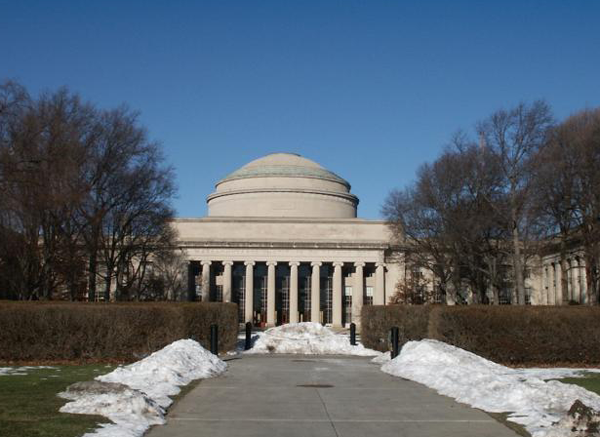
\includegraphics{Figure1}
%  \caption{Teaser Image}
%  \label{fig:teaser}
%}

\maketitle

\begin{abstract}
% TODO
\end{abstract}

% The following section is mandatory for accepted papers, but not needed for submissions for the June 1 deadline.
\keywords{
	Guides; instructions; author's kit; conference publications;
	keywords should be separated by a semi-colon.
}

\category{H.5.m.}{Information Interfaces and Presentation (e.g. HCI)}{Miscellaneous}

See: \url{http://www.acm.org/about/class/1998/}
for more information and the full list of ACM classifiers
and descriptors. 

% The following section can be included for accepted papers, but is not needed for submissions for the June 1 deadline.

\terms{
	Human Factors; Design; Measurement. 
	If you choose more than one ACM General Term, 
	separate the terms with a semi-colon.
}

See list of the limited ACM 16 terms in the
instructions and additional information:
\url{http://www.sheridanprinting.com/sigchi/generalterms.htm}.
% \textcolor{red}{Optional section to be included in your final version.}

\section{Introduction}

% TODO 

\section{Background}

Massive open online courses (MOOCs), such as those currently operated by Coursera, edX, and Udacity, typically include hundreds to thousands of students in each course. Traditional social structures of on-campus courses, such as direct interaction of teachers with each student and hiring teaching assistants to hold small section discussions, become infeasibly expensive at this scale. As Chamberlin and Parish lamented, "The number of people in a course can be overwhelming! How does someone connect with 2000-plus people?"  \cite{Chamberlin:2011:MMO:2016016.2016017} MOOCs exhibit a high level of attrition; \cite{oro36657} the absence of an effective learning community, which has been linked to student attrition, \cite{tinto1993leaving} may be a contributing factor.

A scalable alternative to instructor interaction is interaction among students in an online forum. By exploiting each student's advantages, students can assist one another and create a learning community on their own. This ``peer-to-peer'' learning community model has been pervasive and successful on the web and in online games. \cite{thomas2011new} However, some forums are effective in creating learning communities while others are not, and the chance of success is not directly related to the quantity of posts, but rather is a function of other important metrics such as the quantity of posts with no responses. \cite{quteprints12341} Effective software features in forums can promote the interactions that tend to generate successful learning communities, and discourage those which damage them. The software used by StackOverflow, a popular question-answer website for software developers, contains a number of software mechanisms intended to improve important participation metrics like number of unanswered questions, response time, and overall activity level, and generated a successful learning community. We investigate whether similar features can help to promote a successful student community in the MOOC context.

% \begin{figure}[!h]
% \centering
% 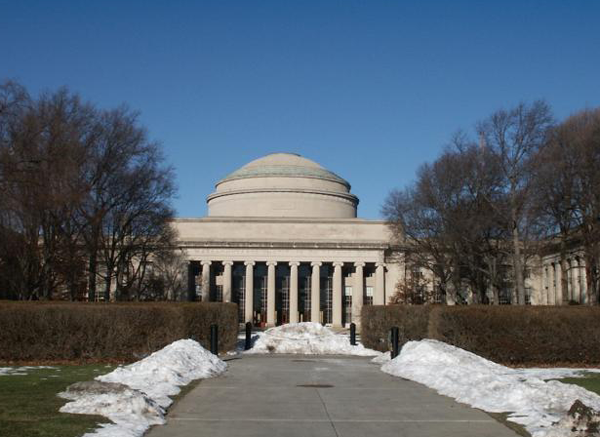
\includegraphics[width=0.9\columnwidth]{Figure1}
% \caption{With Caption Below, be sure to have a good resolution image
%   (see item D within the preparation instructions).}
% \label{fig:figure1}
% \end{figure}

% \begin{table}
%   \centering
%   \begin{tabular}{|c|c|c|}
%     \hline
%     \tabhead{Objects} &
%     \multicolumn{1}{|p{0.3\columnwidth}|}{\centering\tabhead{Caption --- pre-2002}} &
%     \multicolumn{1}{|p{0.4\columnwidth}|}{\centering\tabhead{Caption --- 2003 and afterwards}} \\
%     \hline
%     Tables & Above & Below \\
%     \hline
%     Figures & Below & Below \\
%     \hline
%   \end{tabular}
%   \caption{Table captions should be placed below the table.}
%   \label{tab:table1}
% \end{table}

\section{Conclusion}

% TODO

\section{Acknowledgments}

% TODO

% Balancing columns in a ref list is a bit of a pain because you
% either use a hack like flushend or balance, or manually insert
% a column break.  http://www.tex.ac.uk/cgi-bin/texfaq2html?label=balance
% multicols doesn't work because we're already in two-column mode,
% and flushend isn't awesome, so I choose balance.  See this
% for more info: http://cs.brown.edu/system/software/latex/doc/balance.pdf
%
% Note that in a perfect world balance wants to be in the first
% column of the last page.
%
% If balance doesn't work for you, you can remove that and
% hard-code a column break into the bbl file right before you
% submit:
%
% http://stackoverflow.com/questions/2149854/how-to-manually-equalize-columns-
% in-an-ieee-paper-if-using-bibtex
%
% Or, just remove \balance and give up on balancing the last page.
%
\balance

% If you want to use smaller typesetting for the reference list,
% uncomment the following line:
% \small
\bibliographystyle{acm-sigchi}
\bibliography{forum_experiment_cscw_paper}
\end{document}
